\section{CSI300 point forecasts and residual ablation}
\label{sec:point}
The current CSI300 test contains 1919 forecast origins from 2018-05-03 to 2026-03-30. Results in this section come from \path{results/revised/}. XGBoost uses the configuration and sampling behavior that matched the archived predictions; the current reanalysis reuses the verified first-stage cache, with dates, targets, flags, and hashes checked. HAR, GARCH, DEC, and XGB-AR are re-estimated. Historical outputs remain separate rather than being overwritten.

\subsection{Loss comparisons}
\begin{table}[htbp]\centering
\caption{Revised CSI300 point losses, $N=1919$. MSE and MAE use the log target.}
\label{tab:forecast_metrics}
\begin{tabular}{lrrr}\toprule Model & MSE & MAE & QLIKE\\\midrule
HAR & 4.905206 & 1.724860 & 3.905553\\
GARCH(1,1) & 7.375868 & 1.983865 & 1.564183\\
XGB-Market & 5.099716 & 1.763086 & 4.951636\\
XGB-AR & 5.094169 & 1.758021 & 4.705936\\
DEC & 5.112644 & 1.725558 & 3.536964\\\bottomrule
\end{tabular}
\end{table}

HAR has the lowest log-MSE and MAE, whereas GARCH has the lowest QLIKE. Relative to XGB-Market, DEC reduces QLIKE by approximately 28.57\% and MAE by 2.13\%, but increases MSE by 0.25\%. Thus, the more elaborate correction does not dominate the simpler baselines across losses. Part of the ranking difference reflects the distinction between log-target fitting and direct conditional-variance modeling.

Against XGB-AR, DEC lowers QLIKE from 4.705936 to 3.536964 and MAE from 1.758021 to 1.725558, while raising MSE from 5.094169 to 5.112644. This is a loss-dependent incremental comparison for the EPU component. It does not demonstrate an exogenous policy-uncertainty effect or prove that the monthly inputs were available in real time.

\begin{figure}[htbp]\centering
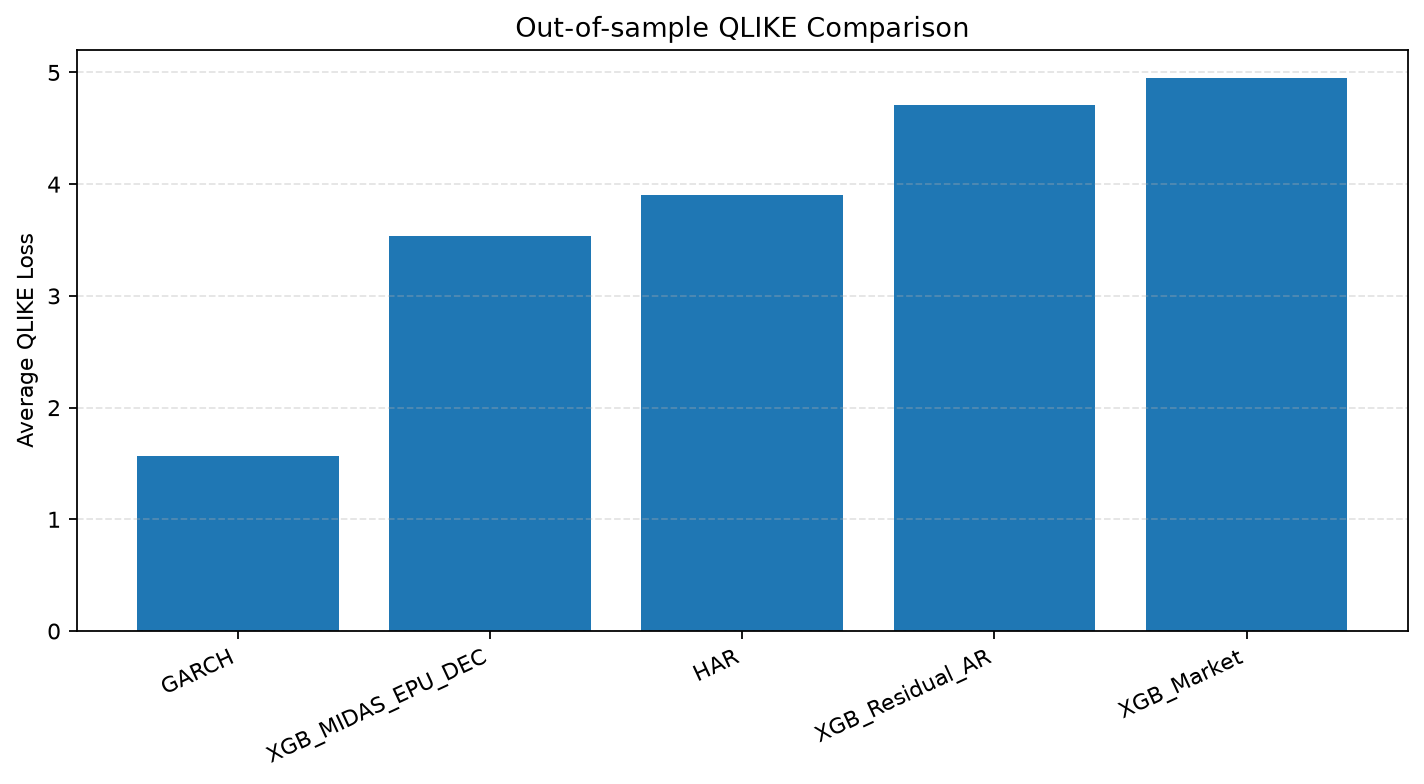
\includegraphics[width=.9\textwidth]{../../results/revised/csi300/fig_metrics_bar.png}
\caption{Revised CSI300 QLIKE across the five models. Lower is better.}
\label{fig:metrics_bar}
\end{figure}

\subsection{Forecast paths and cumulative losses}
Figures~\ref{fig:prediction_series} and~\ref{fig:cumulative_qlike} show recent forecasts and cumulative QLIKE differences. The latter cumulates benchmark loss minus DEC loss. An increase therefore moves the comparison in DEC's favor, but does not show that DEC improves every date or rule out concentration in extreme observations. A smoother prediction path is not by itself evidence of forecasting validity.

\begin{figure}[htbp]\centering
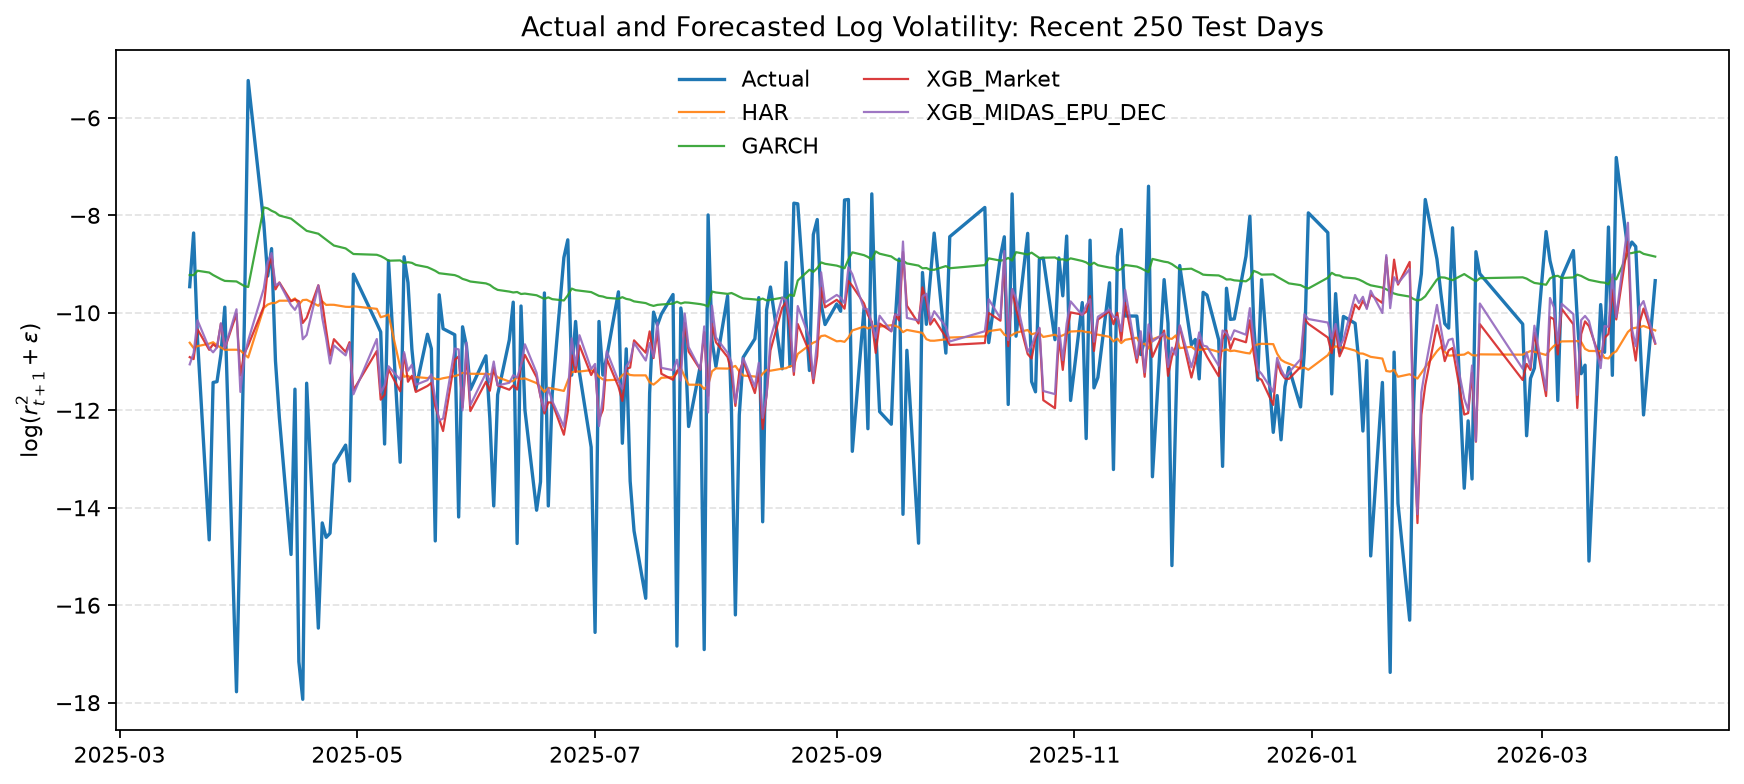
\includegraphics[width=.9\textwidth]{../../results/revised/csi300/fig_prediction_series_recent.png}
\caption{Recent revised DEC forecasts and three market-model benchmarks.}
\label{fig:prediction_series}
\end{figure}
\begin{figure}[htbp]\centering
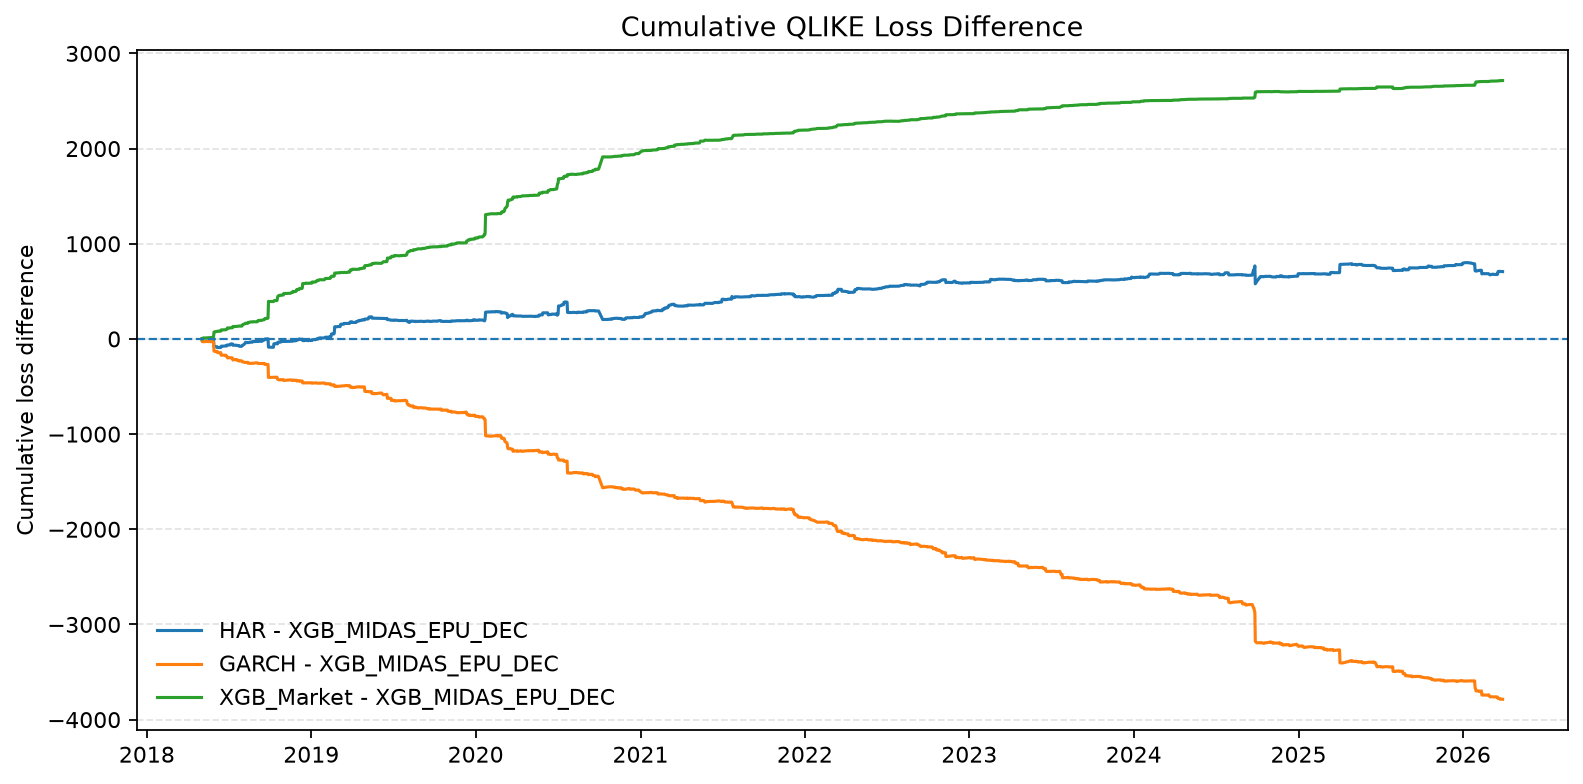
\includegraphics[width=.9\textwidth]{../../results/revised/csi300/fig_cumulative_qlike_diff.png}
\caption{Cumulative CSI300 QLIKE differences: benchmark minus revised DEC.}
\label{fig:cumulative_qlike}
\end{figure}

\subsection{Exploratory loss-difference diagnostics}
Table~\ref{tab:hypothesis_tests} reports the six CSI300 comparisons within the joint 18-comparison Holm adjustment. The reference calculations provide evidence of lower sample MAE and QLIKE relative to the two XGB benchmarks, but not of lower MSE. Their interpretation remains exploratory because of selection, approximate nesting, estimated forecasts, and the retrospective design.

\begin{table}[htbp]\centering\small
\caption{Exploratory CSI300 HAC diagnostics. Positive differences favor DEC.}
\label{tab:hypothesis_tests}
\begin{tabular}{llrrr}\toprule Benchmark & Loss & Mean difference & HAC SE & Holm $p$\\\midrule
XGB-Market & MSE & $-0.012928$ & 0.041430 & 1\\
XGB-Market & MAE & 0.037528 & 0.008207 & $6.73\times10^{-5}$\\
XGB-Market & QLIKE & 1.414672 & 0.197725 & $1.43\times10^{-11}$\\
XGB-AR & MSE & $-0.018475$ & 0.035984 & 1\\
XGB-AR & MAE & 0.032464 & 0.007137 & $7.01\times10^{-5}$\\
XGB-AR & QLIKE & 1.168972 & 0.160859 & $6.61\times10^{-12}$\\\bottomrule
\end{tabular}
\end{table}

\subsection{Selected weights and numerical sensitivity}
CSI300 retains a 24-month exponential Almon specification. Table~\ref{tab:midas_spec} and Figure~\ref{fig:midas_weights} describe the validation-stage choice; test-period parameters are subsequently re-estimated every 60 retained observations. The boundary value of $\theta_1$ indicates that the fitted shape depends on the imposed parameter constraints. These weights should not be interpreted as a stable causal policy-transmission profile.

\begin{table}[htbp]\centering
\caption{CSI300 specification selected by validation MSE.}
\label{tab:midas_spec}
\begin{tabular}{lrrrr}\toprule Family & $K$ & $\theta_1$ & $\theta_2$ & Validation MSE\\\midrule
Exponential Almon & 24 & 5.000000 & $-4.488853$ & 5.722685\\\bottomrule
\end{tabular}
\end{table}
\begin{figure}[htbp]\centering
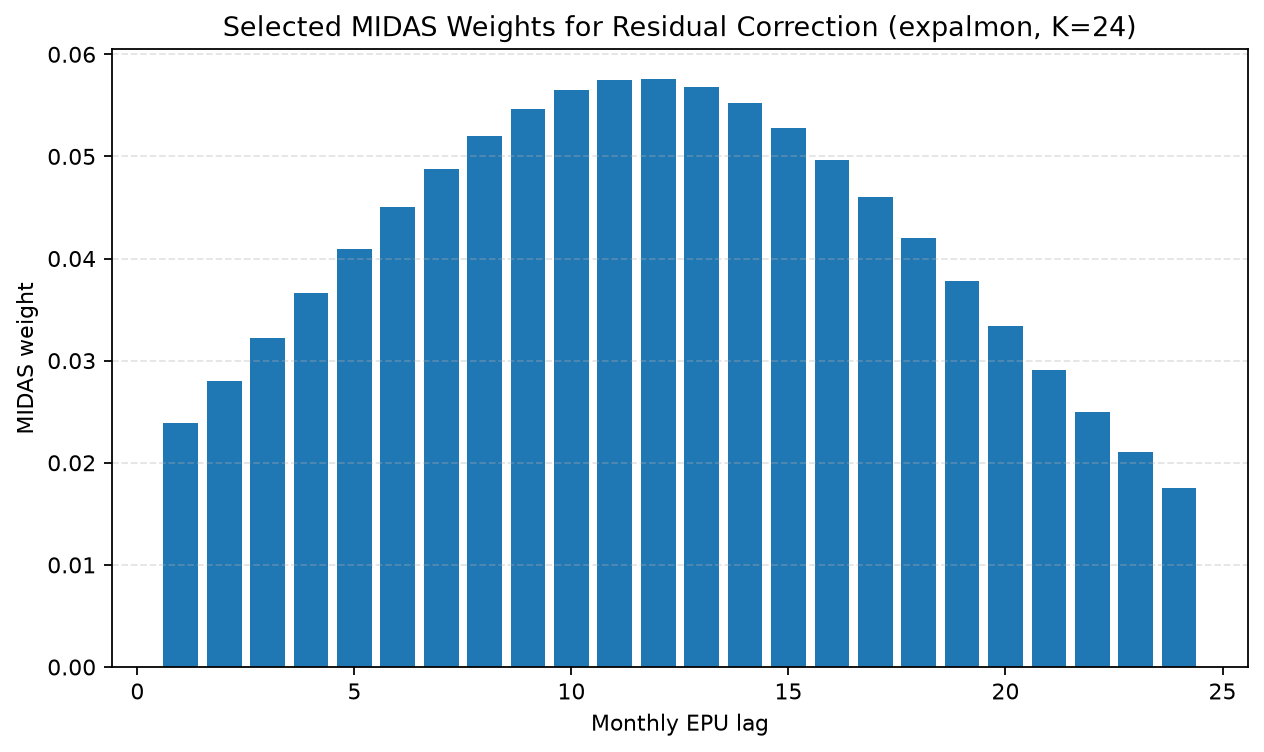
\includegraphics[width=.9\textwidth]{../../results/revised/csi300/fig_midas_weights.png}
\caption{CSI300 MIDAS weights from revised validation selection.}
\label{fig:midas_weights}
\end{figure}

Archived DEC has MSE 5.112383 and QLIKE 3.538317, compared with 5.112644 and 3.536964 after revision. MSE is slightly worse and QLIKE slightly better. The reason for revising the solver is the documented estimation defect and improved numerical diagnostics, not a desire to select the most favorable test scores. Appendix~\ref{app:solver} separates historical reproduction differences from current-method stability checks.
